\documentclass[12pt]{article}
\usepackage[a4paper, bindingoffset=0.2in, %
							left=0.5in,right=0.5in,top=0.5in,bottom=0.5in,%
							footskip=.25in]{geometry}
\usepackage{graphicx}
\usepackage{amsmath}
\usepackage{hyperref}


\title{PSet6 Report}
\author{Ali Abolhassanzadeh Mahani}

\begin{document}
	\maketitle
	\section{Complex Networks}
	The Graphs and theirs degree and clustering distribution is shown in Fig\ref{fig:p1_1} for mean degree 0.8,
	Fig\ref{fig:p1_2} for mean degree 1.0 and Fig\ref{fig:p1_3} for mean degree 8.0.
	\begin{figure}[h!]
		\centering
		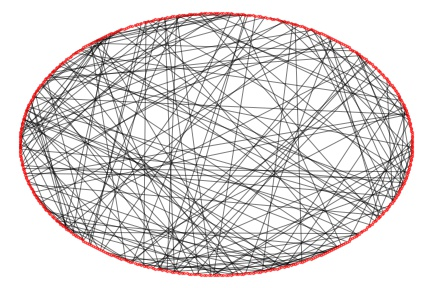
\includegraphics[width=0.4\linewidth]{../p1_0graph.jpg}
		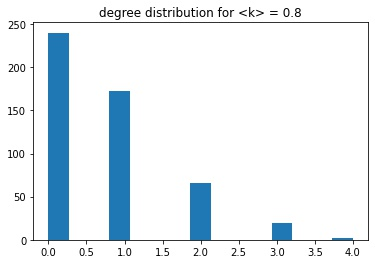
\includegraphics[width=0.4\linewidth]{../p1_0deg.jpg}
		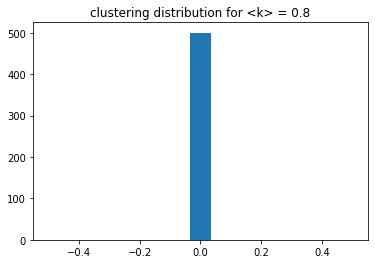
\includegraphics[width=0.4\linewidth]{../p1_0clust.jpg}
		\label{fig:p1_1}
		\caption{Illustrations for graph with mean degree of 0.8}
	\end{figure}

	\begin{figure}[h!]
	\centering
	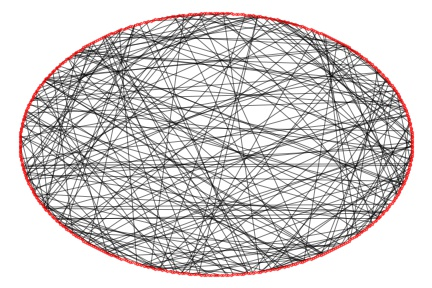
\includegraphics[width=0.4\linewidth]{../p1_1graph.jpg}
	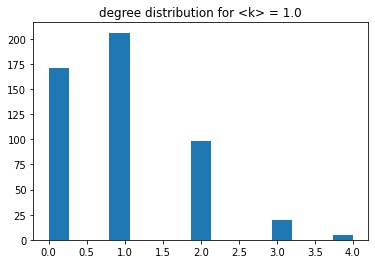
\includegraphics[width=0.4\linewidth]{../p1_1deg.jpg}
	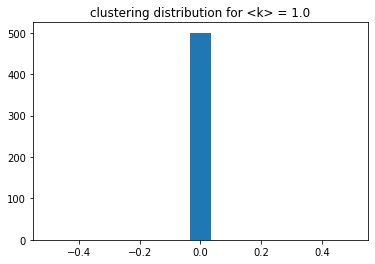
\includegraphics[width=0.4\linewidth]{../p1_1clust.jpg}
	\label{fig:p1_2}
	\caption{Illustrations for graph with mean degree of 1.0}
\end{figure}

	\begin{figure}[h!]
	\centering
	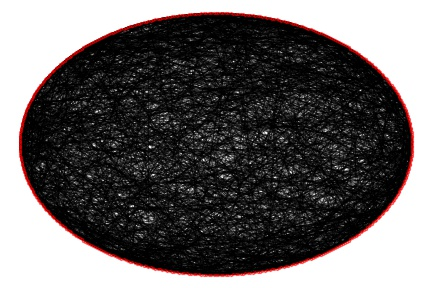
\includegraphics[width=0.4\linewidth]{../p1_8graph.jpg}
	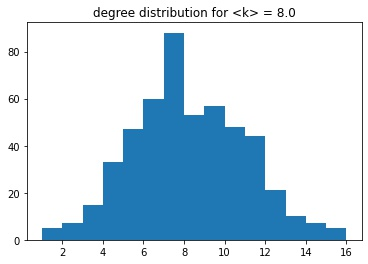
\includegraphics[width=0.4\linewidth]{../p1_8deg.jpg}
	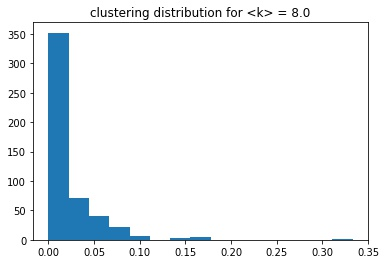
\includegraphics[width=0.4\linewidth]{../p1_8clust.jpg}
	\label{fig:p1_3}
	\caption{Illustrations for graph with mean degree of 8.0}
\end{figure}

	\section{Monte Carlo Integral(SS MC \& IS MC)}
	I did the SS MC and IS MC as wanted. I defined their functions and used \texttt{time.time()} to find the 
	runtime of the integration. The results are available in Table\ref{tab:MC}\\
	It's worth noting that the numeric value is roughly $0.8820814$
	\begin{table}[h!]
		\centering
		\begin{tabular}{|c|c|c|c|c||c|c|c|c|}
			\hline
			n & \multicolumn{4}{|c||}{SS MC} & \multicolumn{4}{|c|}{IS MC} \\
			\hline
			n & I & $\Delta_{stat} I$ & $\Delta_{real} I$ & $t$ & I & $\Delta_{stat} I$ & $\Delta_{real} I$ & $t$ \\
			\hline
 			$1000$ & $0.858522$ & $0.546$ & $0.023$ & $0.02078$ & $0.882866$ & $0.0100$ & $0.00078$ & $0.01938$ \\
 			\hline
			 $2000$ & $0.861797$ & $0.55$ & $0.02$ & $0.01930$ & $0.871512$ & $0.007$ & $0.0106$ & $0.03906$ \\
			 \hline
			 $4000$ & $0.884244$ & $0.56$ & $0.0022$ & $0.05336$ & $0.875264$ & $0.005$ & $0.007$ & $0.08817$ \\
			 \hline
			 $8000$ & $0.886907$ & $0.56$ & $0.0048$ & $0.07861$ & $0.883804$ & $0.003$ & $0.002$ & $0.11154$ \\
			 \hline
			 $16000$ & $0.883410$ & $0.560$ & $0.0013$ & $0.14961$ & $0.882986$ & $0.002$ & $0.0009$ & $0.20379$ \\
			 \hline
			 $32000$ & $0.875776$ & $0.557$ & $0.0063$ & $0.19460$ & $0.881274$ & $0.0017$ & $0.0008$ & $0.39223$ \\
			 \hline
			 $64000$ & $0.879419$ & $0.558$ & $0.0027$ & $0.33243$ & $0.881791$ & $0.0012$ & $0.0003$ & $0.69962$ \\
			 \hline
		\end{tabular}
	\label{tab:MC}
	\caption{Data for numerical integration using SS MC and IS MC.}	
	\end{table}
	\section{The Sphere (Multi variable Integration SS MC)}
	
	\section{Metropolis Random Generation}
	
	
	
\end{document}